\chapter{Burning: What a Fire Needs}\label{ch:g4:what-a-fire-needs}

A campfire at dusk. It needed dry wood, a match to start it, and the
wind that blows through it keeps it bright. After an hour, the logs have
shrunk to glowing embers and white ash, and grey smoke has drifted away
into the sky. Where has the wood gone? What does a fire need, and what
does it leave behind?

\begin{recall}
\omterm{def:g4:air-a-mixture-of-gases:air}{Air} is a mixture of gases: about four fifths nitrogen and one fifth
oxygen, with a little argon and carbon dioxide. A flame takes oxygen from
the \omterm{def:g4:air-a-mixture-of-gases:air}{air} around it; a candle under a jar goes out when too little oxygen
is left (\cref{ch:g4:air-a-mixture-of-gases}).
\end{recall}

\begin{omfigure}
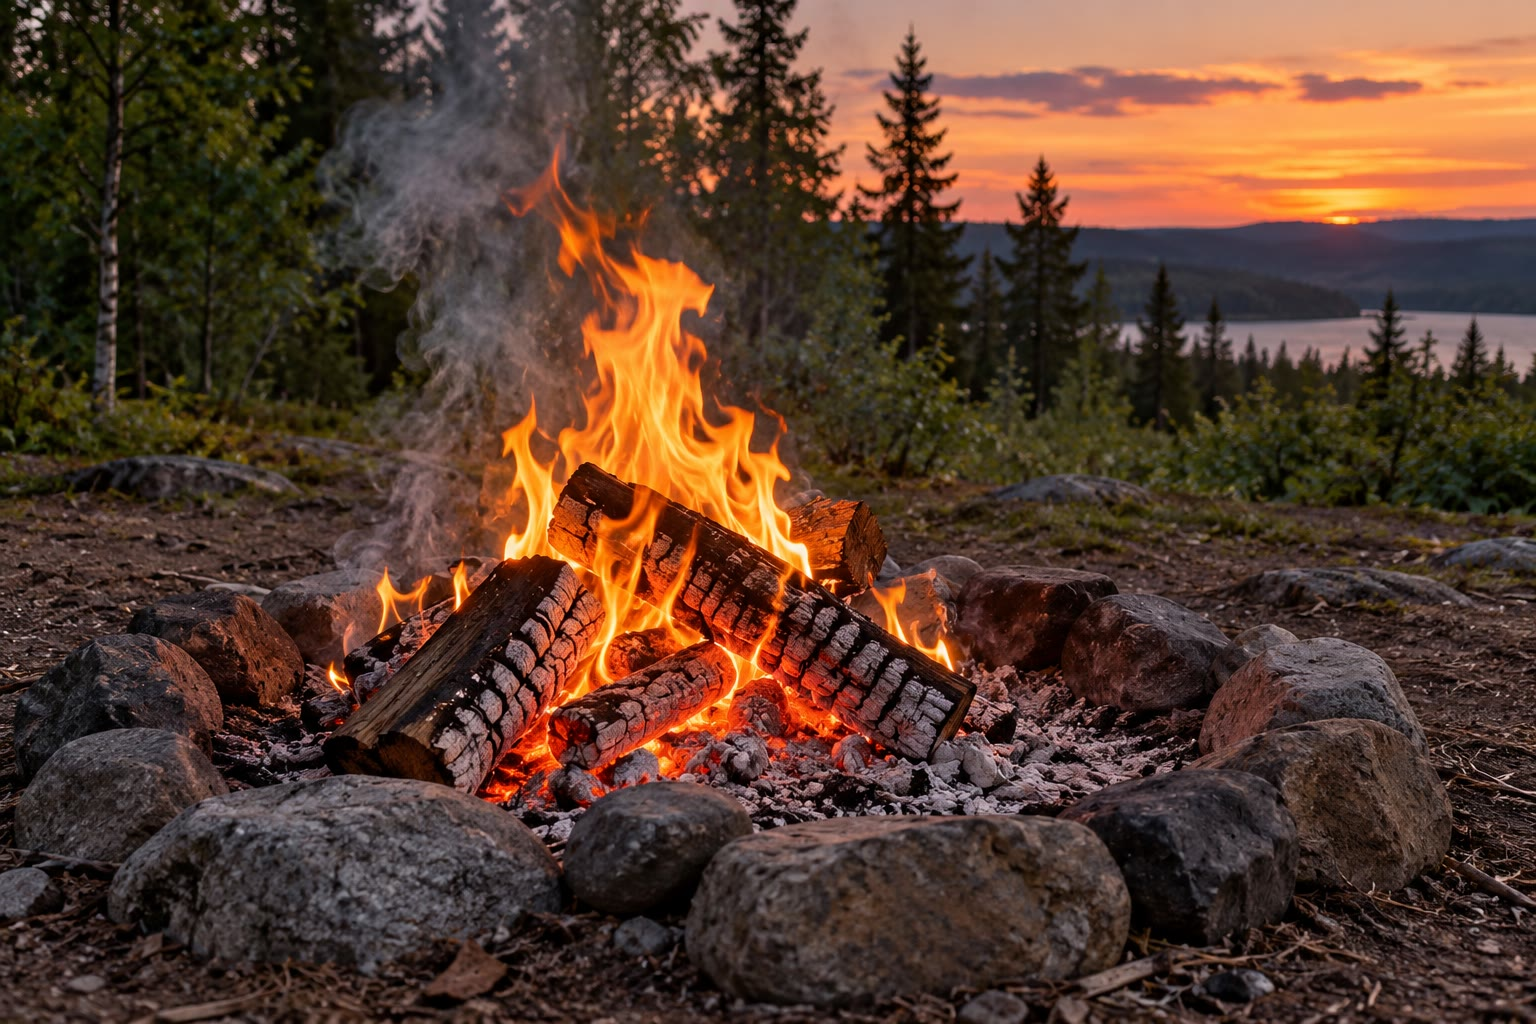
\includegraphics[width=0.6\linewidth]{images/book1/ai/g4-campfire.jpg}

{\small A campfire: wood, \omterm{def:g4:air-a-mixture-of-gases:air}{air} and a match --- and afterwards ash and
smoke.}
\end{omfigure}

\section{Fuels}

\begin{definition}[Fuel]\label{def:g4:what-a-fire-needs:fuel}
A \emph{fuel}\index{fuel} is a material that can burn and give out heat
and light: wood, paper, coal, candle wax, the gas of a cooker, petrol,
heating oil.
\end{definition}

\begin{example}[Solid, liquid and gas fuels]\label{ex:g4:what-a-fire-needs:fuels}
Wood, paper, coal and candle wax are solid \omterm{def:g4:what-a-fire-needs:fuel}{fuels}. Petrol and heating oil
are liquid \omterm{def:g4:what-a-fire-needs:fuel}{fuels}. The gas of a kitchen cooker and the gas in a lighter
are gas \omterm{def:g4:what-a-fire-needs:fuel}{fuels}.
\end{example}

\begin{remark}[Not everything burns]\label{rem:g4:what-a-fire-needs:not}
Stone, sand, glass and water do not burn: they are not \omterm{def:g4:what-a-fire-needs:fuel}{fuels}. That is
why a fireplace is built of stone or brick, and why sand and water are
used to put fires out.
\end{remark}

\section{The fire triangle}

\begin{definition}[Fire triangle]\label{def:g4:what-a-fire-needs:fire-triangle}
A fire needs three things at the same time: a \omterm{def:g4:what-a-fire-needs:fuel}{fuel}, oxygen from the \omterm{def:g4:air-a-mixture-of-gases:air}{air},
and heat to start it. These three things are drawn as the three sides of
a triangle, the \emph{fire triangle}\index{fire triangle}. If one side
is missing, there is no fire.
\end{definition}

\begin{omfigure}
\begin{tikzpicture}[font=\small]
  \coordinate (A) at (0,0); \coordinate (B) at (5,0); \coordinate (C) at (2.5,4.1);
  \draw[line width=3pt, brown!70!black] (A) -- (B);
  \draw[line width=3pt, omDef] (B) -- (C);
  \draw[line width=3pt, red!75!black] (C) -- (A);
  \node[below=4pt, font=\small\bfseries, brown!60!black] at (2.5,0) {fuel};
  \node[right=4pt, font=\small\bfseries, omDef] at (3.75,2.05) {oxygen (from the air)};
  \node[left=4pt, font=\small\bfseries, red!75!black] at (1.25,2.05) {heat (to start)};
  % a flame in the middle
  \fill[orange!80] (2.5,0.55) .. controls (1.95,1.15) and (2.35,1.75) .. (2.55,2.3)
    .. controls (2.75,1.75) and (3.05,1.15) .. (2.5,0.55);
  \fill[yellow!80] (2.5,0.7) .. controls (2.25,1.05) and (2.4,1.35) .. (2.52,1.65)
    .. controls (2.62,1.35) and (2.75,1.05) .. (2.5,0.7);
\end{tikzpicture}

{\small The \omterm{def:g4:what-a-fire-needs:fire-triangle}{fire triangle}: \omterm{def:g4:what-a-fire-needs:fuel}{fuel}, oxygen and heat, all three together.}
\end{omfigure}

\begin{example}[Lighting a match]\label{ex:g4:what-a-fire-needs:match}
A match head is rubbed on the side of its box. The rubbing heats it
enough to start it \omterm{def:g4:what-a-fire-needs:burning}{burning}: the heat side of the triangle. The wood of
the match is the \omterm{def:g4:what-a-fire-needs:fuel}{fuel}, and the \omterm{def:g4:air-a-mixture-of-gases:air}{air} brings the oxygen.
\end{example}

\begin{example}[Blowing on embers]\label{ex:g4:what-a-fire-needs:embers}
Glowing embers that seem almost dead burst into flame again when
someone blows on them: the blowing brings more \omterm{def:g4:air-a-mixture-of-gases:air}{air}, and so more oxygen,
to the \omterm{def:g4:what-a-fire-needs:fuel}{fuel} that is still hot.
\end{example}

\section{Burning makes new substances}

\begin{definition}[Burning and combustion]\label{def:g4:what-a-fire-needs:burning}
\emph{Burning}\index{burning} is what happens when a \omterm{def:g4:what-a-fire-needs:fuel}{fuel} takes oxygen
from the \omterm{def:g4:air-a-mixture-of-gases:air}{air} and gives out heat and light. Chemists call a burning a
\emph{combustion}\index{combustion}. During a combustion the \omterm{def:g4:what-a-fire-needs:fuel}{fuel} and
the oxygen are used up, and new substances appear: smoke, ash, carbon
dioxide and water vapour.
\end{definition}

\begin{proposition}[A burning cannot be undone]\label{prop:g4:what-a-fire-needs:new}
The ash and smoke of a fire do not turn back into wood, however long we
wait. \omterm{def:g4:what-a-fire-needs:burning}{Burning} makes new substances that were not there before; the \omterm{def:g4:what-a-fire-needs:fuel}{fuel}
is gone for good.
\end{proposition}

\begin{inthelab}[A cold glass over a candle]
The teacher holds a cold, dry glass beaker upside down for a moment above
a candle flame. The inside of the glass mists up with tiny droplets of
water: water vapour made by the \omterm{def:g4:what-a-fire-needs:burning}{burning} candle has turned back into
liquid on the cold glass. A \omterm{def:g4:what-a-fire-needs:burning}{burning} candle makes water, and carbon
dioxide too, which can be detected with a test met in a later chapter.
\end{inthelab}

\begin{omfigure}
\begin{tikzpicture}[font=\small, scale=1.3]
  % candle
  \fill[white, draw=black!50] (-0.25,0) rectangle (0.25,1.2);
  \draw[black!70] (0,1.2) -- (0,1.33);
  \fill[orange!85] (0,1.3) .. controls (-0.16,1.5) and (-0.06,1.75) .. (0,1.95)
    .. controls (0.06,1.75) and (0.16,1.5) .. (0,1.3);
  \fill[yellow!85] (0,1.36) .. controls (-0.08,1.5) and (-0.03,1.62) .. (0,1.72)
    .. controls (0.03,1.62) and (0.08,1.5) .. (0,1.36);
  % upturned cold beaker above
  \pic[transform shape, rotate=180] at (0,4.3) {beaker={0}{white}};
  \foreach \x/\y in {-0.6/3.9,-0.45/4.1,-0.2/3.95,0.1/4.15,0.35/3.9,0.6/4.05,
                     -0.7/3.5,0.7/3.4,-0.72/3.0,0.72/2.9}
    \fill[omDef!55] (\x,\y) circle (0.035);
  \draw[<-, omProp, thick] (0.68,3.95) -- (2.0,4.2) node[right, text=black]
    {droplets of water};
  \draw[<-, omProp, thick] (0.85,3.2) -- (2.0,3.3) node[right, text=black]
    {cold glass, upside down};
  \draw[<-, omProp, thick] (0.15,1.7) -- (2.0,1.9) node[right, text=black]
    {the flame: wax burning};
  \draw[<-, omProp, thick] (0.3,0.6) -- (2.0,0.7) node[right, text=black]
    {candle wax: the fuel};
\end{tikzpicture}

{\small A cold glass held above a candle mists up: \omterm{def:g4:what-a-fire-needs:burning}{burning} wax makes
water vapour.}
\end{omfigure}

\begin{example}[What a log becomes]\label{ex:g4:what-a-fire-needs:log}
A log of a few kilograms burns down to a small heap of ash. Most of the
wood has not vanished: together with oxygen from the \omterm{def:g4:air-a-mixture-of-gases:air}{air}, it has become
smoke, carbon dioxide and water vapour, which are gases and drift away
into the sky.
\end{example}

\section{Putting a fire out}

\begin{method}[Putting out a fire: take away one side]\label{met:g4:what-a-fire-needs:out}
To put out a fire, take away one side of the \omterm{def:g4:what-a-fire-needs:fire-triangle}{fire triangle}:
\begin{itemize}
  \item \textbf{take away the oxygen}: cover the fire with a fire
        blanket, a lid or sand, so that \omterm{def:g4:air-a-mixture-of-gases:air}{air} cannot reach it;
  \item \textbf{take away the heat}: pour water on \omterm{def:g4:what-a-fire-needs:burning}{burning} wood or
        paper, which cools it below the point where it can burn;
  \item \textbf{take away the \omterm{def:g4:what-a-fire-needs:fuel}{fuel}}: turn off the gas tap, or clear the
        dry plants around a forest fire.
\end{itemize}
\end{method}

\begin{omfigure}
\begin{tikzpicture}[font=\small, scale=0.7]
  \foreach \k/\lab/\side in {0/{a blanket: no oxygen}/1, 1/{water: no heat}/2,
                              2/{gas turned off: no fuel}/0} {
    \begin{scope}[xshift=\k*6.2cm]
      \coordinate (A) at (0,0); \coordinate (B) at (4,0); \coordinate (C) at (2,3.3);
      \pgfmathsetmacro\oa{\side==0 ? 0.2 : 1}
      \pgfmathsetmacro\ob{\side==1 ? 0.2 : 1}
      \pgfmathsetmacro\oc{\side==2 ? 0.2 : 1}
      \draw[line width=2.5pt, brown!70!black, opacity=\oa] (A) -- (B);
      \draw[line width=2.5pt, omDef, opacity=\ob] (B) -- (C);
      \draw[line width=2.5pt, red!75!black, opacity=\oc] (C) -- (A);
      \ifnum\side=0 \draw[line width=1.4pt, black] (1.6,-0.4) -- (2.4,0.4) (1.6,0.4) -- (2.4,-0.4);\fi
      \ifnum\side=1 \draw[line width=1.4pt, black] (2.6,1.25) -- (3.4,2.05) (2.6,2.05) -- (3.4,1.25);\fi
      \ifnum\side=2 \draw[line width=1.4pt, black] (0.6,1.25) -- (1.4,2.05) (0.6,2.05) -- (1.4,1.25);\fi
      \node[align=center, anchor=north] at (2,-0.6) {\lab};
    \end{scope}
  }
\end{tikzpicture}

{\small Three ways to put out a fire, each removing one side of the
triangle (crossed out): the oxygen, the heat or the \omterm{def:g4:what-a-fire-needs:fuel}{fuel}.}
\end{omfigure}

\begin{omfigure}
\begin{minipage}[t]{0.48\linewidth}\centering
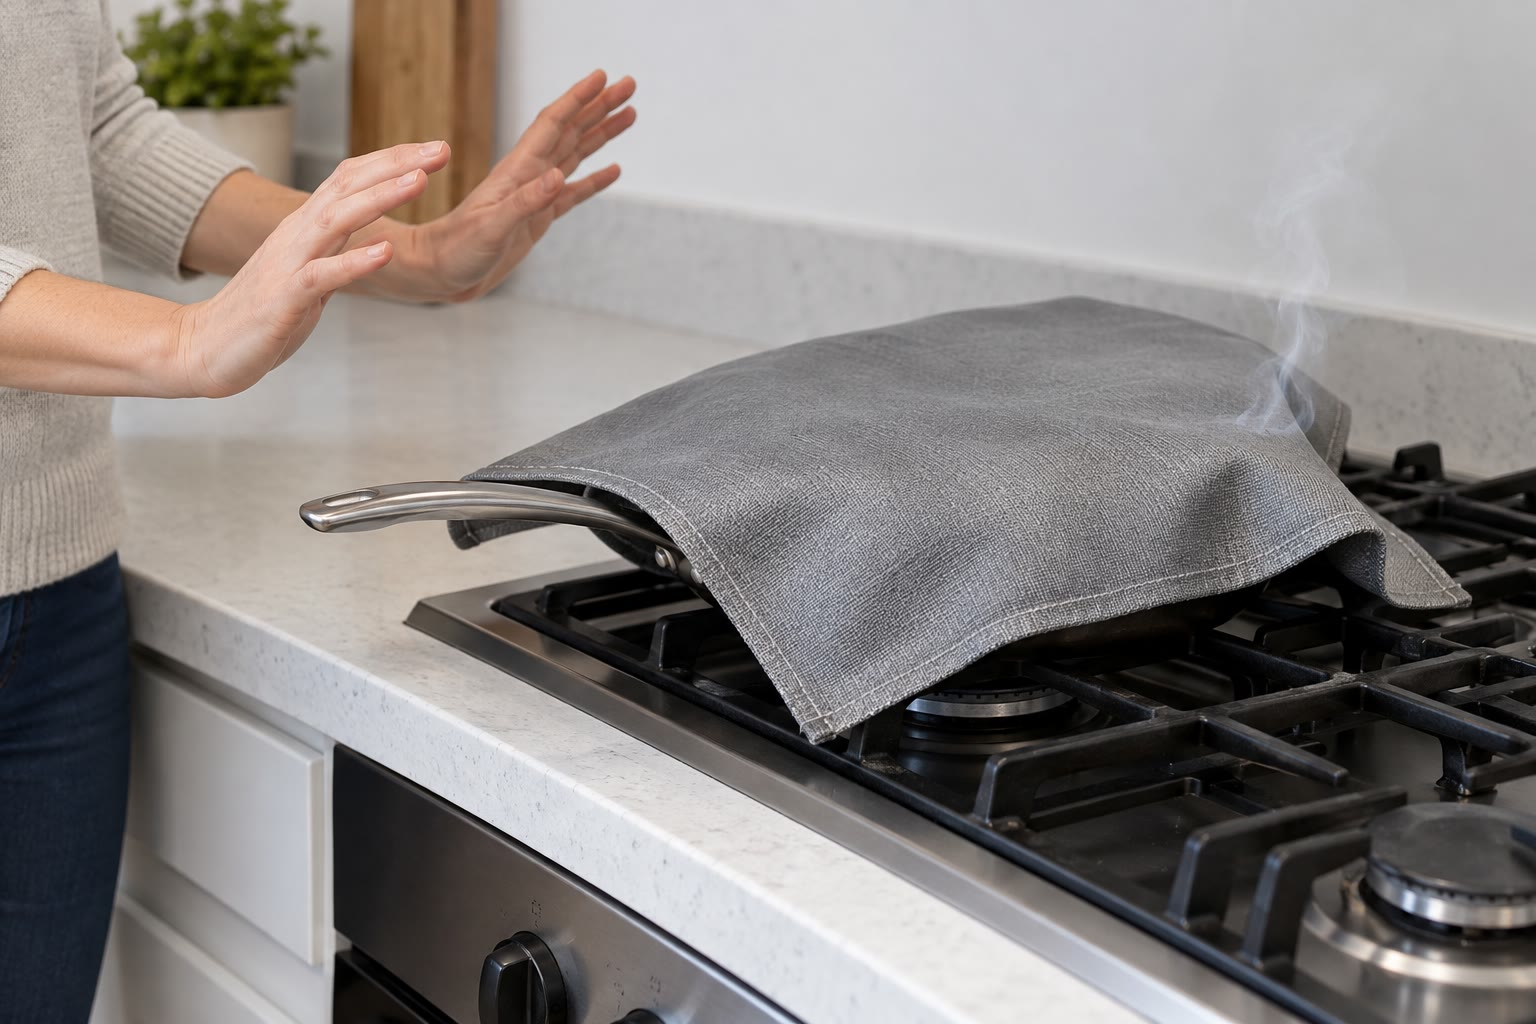
\includegraphics[width=\linewidth,height=4.6cm,keepaspectratio]{images/book1/ai/g4-fire-blanket.jpg}

{\small A fire blanket over a pan: the \omterm{def:g4:air-a-mixture-of-gases:air}{air} can no longer reach the
fire.}
\end{minipage}\hfill
\begin{minipage}[t]{0.48\linewidth}\centering
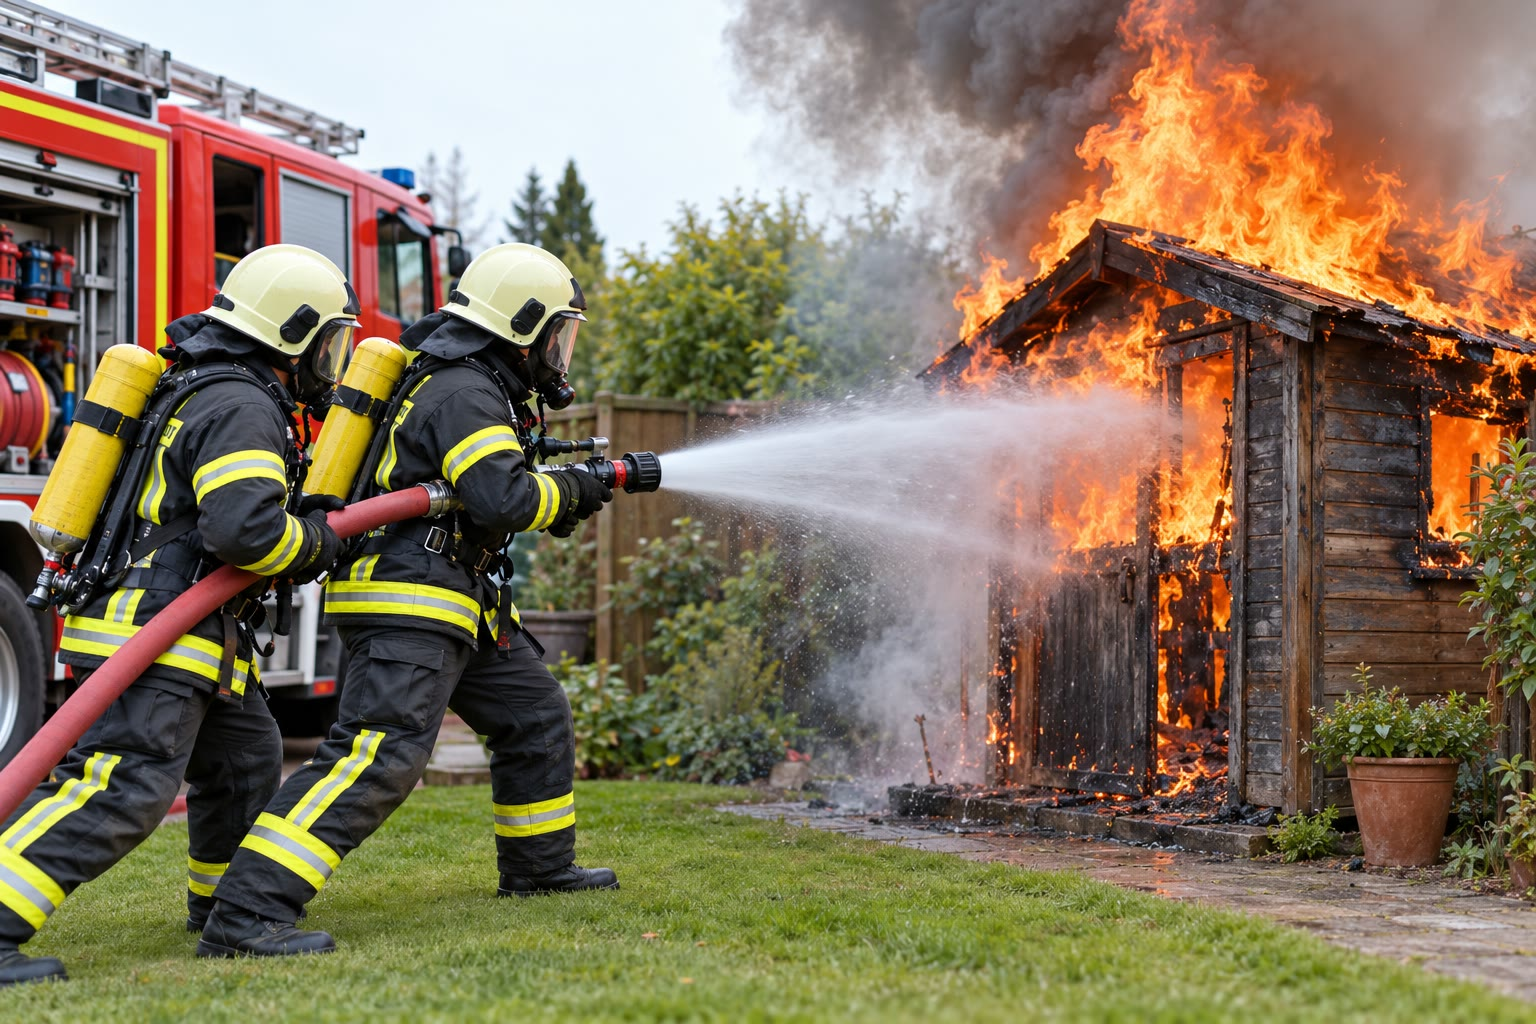
\includegraphics[width=\linewidth,height=4.6cm,keepaspectratio]{images/book1/ai/g4-firefighters.jpg}

{\small Firefighters spray water to cool a \omterm{def:g4:what-a-fire-needs:burning}{burning} shed.}
\end{minipage}
\end{omfigure}

\section{Fire safety}

\begin{remark}[Never water on a pan of burning oil]\label{rem:g4:what-a-fire-needs:oil}
If the oil in a frying pan catches fire, nobody should throw water on
it: the water boils at once under the oil and throws \omterm{def:g4:what-a-fire-needs:burning}{burning} oil out of
the pan. The gas or the hotplate is turned off and the pan is covered
with a lid or a fire blanket, by an adult.
\end{remark}

\begin{safety}{\ghs{GHS02}\ghs{GHS04}}
% ledger: ghs:butane
The gas in a lighter or a camping cartridge is butane. Its flame
pictogram (GHS02) means: extremely flammable, keep away from flames and
sparks. The gas bottle pictogram (GHS04) means: a gas kept under
pressure.
\end{safety}

\begin{proposition}[What to do if there is a fire]\label{prop:g4:what-a-fire-needs:safety}
Smoke is the first danger of a fire: it is hot, it hides the way out and
it is poisonous to breathe. A smoke alarm on the ceiling beeps loudly
as soon as smoke reaches it. If there is a fire: get out, keep low under
the smoke, close the doors behind you, and call the fire brigade from
outside. Never go back in.
\end{proposition}

\begin{omfigure}
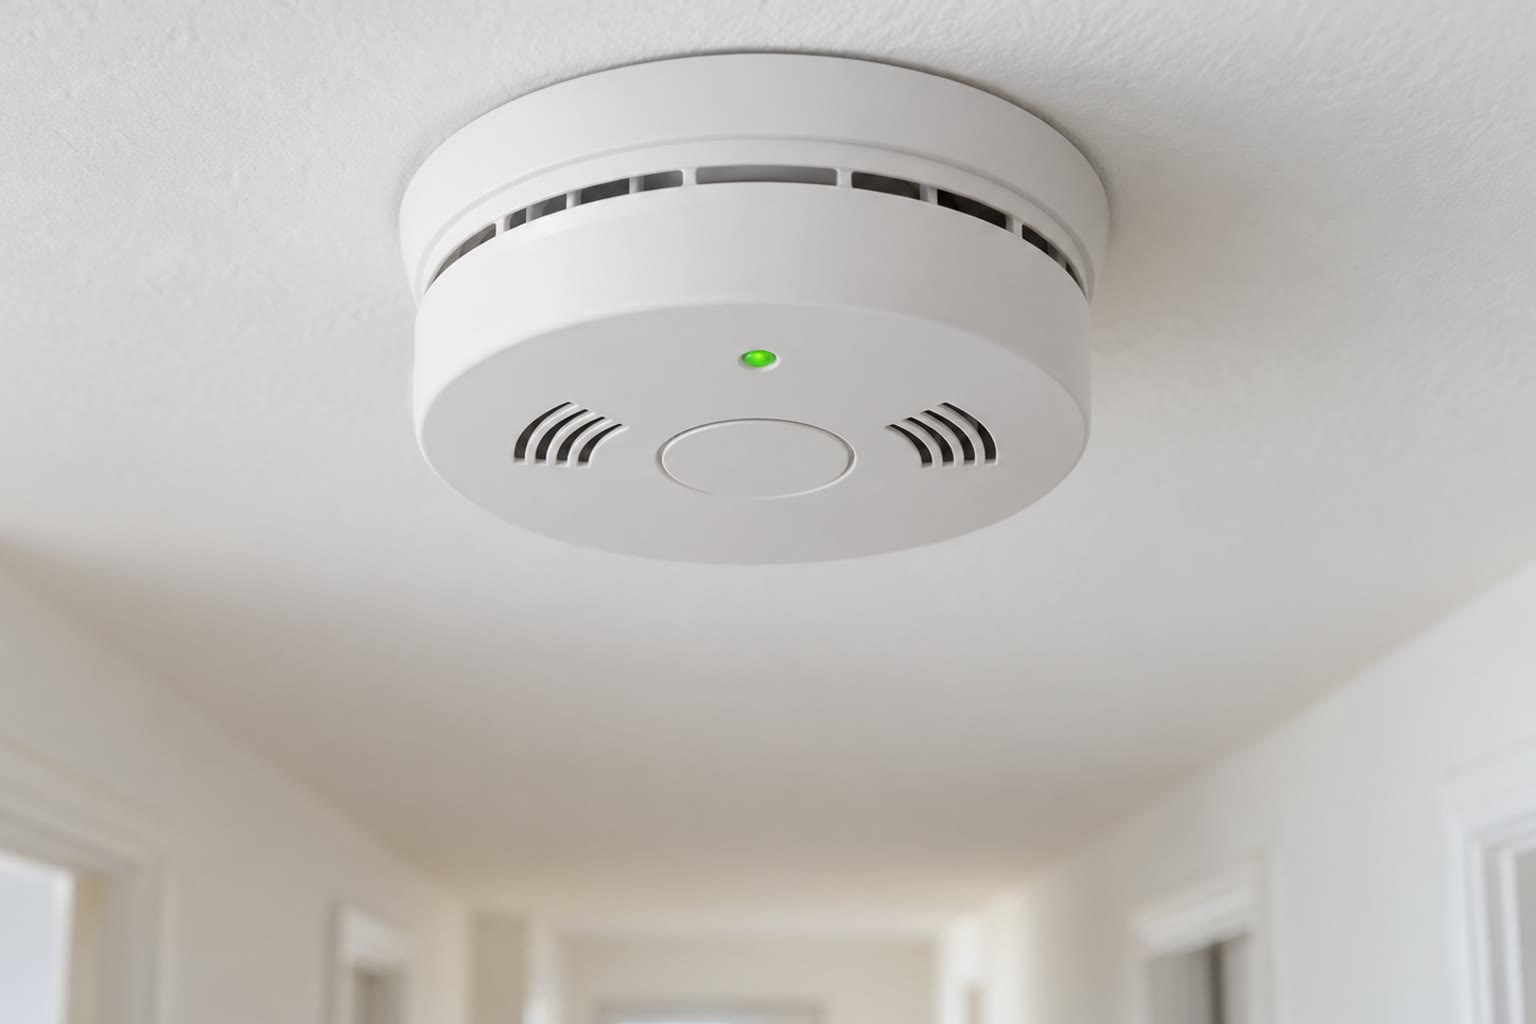
\includegraphics[width=0.42\linewidth]{images/book1/ai/g4-smoke-alarm.jpg}

{\small A smoke alarm: it sounds as soon as smoke reaches it.}
\end{omfigure}

\section{Exercises}

\begin{exercise}[$\star$]\label{exo:g4:what-a-fire-needs:1}
Name the three sides of the \omterm{def:g4:what-a-fire-needs:fire-triangle}{fire triangle}.
\end{exercise}

\begin{exercise}[$\star$]\label{exo:g4:what-a-fire-needs:2}
Which of these are \omterm{def:g4:what-a-fire-needs:fuel}{fuels}: wood, sand, candle wax, glass, petrol, water,
paper?
\end{exercise}

\begin{exercise}[$\star$]\label{exo:g4:what-a-fire-needs:3}
A fire blanket is thrown over a small fire. Which side of the \omterm{def:g4:what-a-fire-needs:fire-triangle}{fire
triangle} does it take away?
\end{exercise}

\begin{exercise}[$\star$]\label{exo:g4:what-a-fire-needs:4}
Firefighters spray water on a \omterm{def:g4:what-a-fire-needs:burning}{burning} shed. Which side of the \omterm{def:g4:what-a-fire-needs:fire-triangle}{fire
triangle} does the water take away?
\end{exercise}

\begin{exercise}[$\star$]\label{exo:g4:what-a-fire-needs:5}
Name three new substances made when wood burns.
\end{exercise}

\begin{exercise}[$\star$]\label{exo:g4:what-a-fire-needs:6}
Why does blowing on glowing embers make them flare up again?
\end{exercise}

\begin{exercise}[$\star$]\label{exo:g4:what-a-fire-needs:7}
A cold glass held above a candle mists up. Which new substance has the
candle made?
\end{exercise}

\begin{exercise}[$\star$]\label{exo:g4:what-a-fire-needs:8}
What should you do first if a smoke alarm goes off and you see smoke?
\end{exercise}

\begin{exercise}[$\star$]\label{exo:g4:what-a-fire-needs:9}
Look at the figure with the three small triangles. Which side is crossed
out when the gas is turned off?
\end{exercise}

\begin{exercise}[$\star\star$]\label{exo:g4:what-a-fire-needs:10}
To stop a forest fire, firefighters sometimes cut down a wide strip of
trees in front of it. Which side of the \omterm{def:g4:what-a-fire-needs:fire-triangle}{fire triangle} are they taking
away?
\end{exercise}

\begin{exercise}[$\star\star$]\label{exo:g4:what-a-fire-needs:11}
A log weighs much more than its ash. Has part of the log disappeared?
Explain where it has gone.
\end{exercise}
